% Dedicated to Craig Leto
\documentclass{article}
\RequirePackage{amsmath}
\RequirePackage{bytefield}
\RequirePackage{graphicx}
\RequirePackage{newtxmath}
\RequirePackage{mathtools}
\RequirePackage{xspace}
\RequirePackage{url}
\RequirePackage{changepage}
\RequirePackage{enumitem}
\RequirePackage{tabularx}
\RequirePackage{hhline}
\RequirePackage[usestackEOL]{stackengine}
\RequirePackage{comment}
\RequirePackage{needspace}
\RequirePackage[nobottomtitles]{titlesec}
\RequirePackage[hang]{footmisc}
\RequirePackage{xstring}
\RequirePackage[unicode,bookmarksnumbered,bookmarksopen,pdfview=Fit]{hyperref}
\RequirePackage{cleveref}
\RequirePackage{nameref}

\RequirePackage[style=alphabetic,maxbibnames=99,dateabbrev=false,urldate=iso8601,backref=true,backrefstyle=none,backend=biber]{biblatex}
\addbibresource{sietch.bib}

% Fonts
\RequirePackage{lmodern}
\RequirePackage{quattrocento}
\RequirePackage[bb=ams]{mathalfa}

% Quattrocento is beautiful but doesn't have an italic face. So we scale
% New Century Schoolbook italic to fit in with slanted Quattrocento and
% match its x height.
\renewcommand{\emph}[1]{\hspace{0.15em}{\fontfamily{pnc}\selectfont\scalebox{1.02}[0.999]{\textit{#1}}}\hspace{0.02em}}

% While we're at it, let's match the tt x height to Quattrocento as well.
\let\oldtexttt\texttt
\let\oldmathtt\mathtt
\renewcommand{\texttt}[1]{\scalebox{1.02}[1.07]{\oldtexttt{#1}}}
\renewcommand{\mathtt}[1]{\scalebox{1.02}[1.07]{$\oldmathtt{#1}$}}

\newcommand{\zsendmany}{\textbf{z\_sendmany}}

% bold but not extended
\newcommand{\textbnx}[1]{{\fontseries{b}\selectfont #1}}


\crefformat{footnote}{#2\footnotemark[#1]#3}

\DeclareLabelalphaTemplate{
  \labelelement{\field{citekey}}
}

\DefineBibliographyStrings{english}{
  page  = {page},
  pages = {pages},
  backrefpage = {\mbox{$\uparrow$ p\!}},
  backrefpages = {\mbox{$\uparrow$ p\!}}
}

\setlength{\oddsidemargin}{-0.25in}
\setlength{\textwidth}{7in}
\setlength{\topmargin}{-0.75in}
\setlength{\textheight}{9.2in}
\setlength{\parindent}{0ex}
\renewcommand{\arraystretch}{1.4}
\overfullrule=2cm

\setlength{\footnotemargin}{0.6em}
\setlength{\footnotesep}{2ex}
\addtolength{\skip\footins}{3ex}

\renewcommand{\bottomtitlespace}{8ex}

% Use rubber lengths between paragraphs to improve default pagination.
% https://tex.stackexchange.com/questions/17178/vertical-spacing-pagination-and-ideal-results
\setlength{\parskip}{1.5ex plus 1pt minus 1pt}

\setlist[enumerate]{before=\vspace{-1ex}}
\setlist[itemize]{itemsep=0.5ex,topsep=0.2ex,before=\vspace{-1ex},after=\vspace{1.5ex}}

\newlist{formulae}{itemize}{3}
\setlist[formulae]{itemsep=0.2ex,topsep=0ex,leftmargin=1.5em,label=,after=\vspace{1.5ex}}

\newcommand{\docversion}{Whitepaper Version 0.4}
\newcommand{\termbf}[1]{\textbf{#1}\xspace}
\newcommand{\Hushlist}{\termbf{HushList}}
\newcommand{\HushList}{\termbf{HushList}}
\newcommand{\Hushlists}{\termbf{HushLists}}
\newcommand{\HushLists}{\termbf{HushLists}}

\newcommand{\doctitle}{Attacking Zcash Protocol For Fun And Profit}
\newcommand{\leadauthor}{Duke Leto + The Hush Developers}

\newcommand{\keywords}{anonymity, zcash protocol, cryptographic protocols, zk-SNARKs, metadata leakage, de-anonymization,\
electronic commerce and payment, financial privacy, zero knowledge mathematics,\
linkability, transaction graphs, shielded transactions, blockchain analysis }

\hypersetup{
  pdfborderstyle={/S/U/W 0.7},
  pdfinfo={
    Title={\doctitle, \docversion},
    Author={\leadauthor},
    Keywords={\keywords}
  }
}

\makeatletter
\renewcommand*{\@fnsymbol}[1]{\ensuremath{\ifcase#1\or \dagger\or \ddagger\or
    \mathsection\or \mathparagraph\else\@ctrerr\fi}}
\makeatother

\renewcommand{\sectionautorefname}{\S\!}
\renewcommand{\subsectionautorefname}{\S\!}
\renewcommand{\subsubsectionautorefname}{\S\!}
\renewcommand{\subparagraphautorefname}{\S\!}
\newcommand{\crossref}[1]{\autoref{#1}\, \emph{`\nameref*{#1}\kern -0.05em'} on p.\,\pageref*{#1}}

\newcommand{\nstrut}[1]{\texorpdfstring{#1\rule[-.2\baselineskip]{0pt}{\baselineskip}}{#1}}
\newcommand{\nsection}[1]{\section{\nstrut{#1}}}
\newcommand{\nsubsection}[1]{\subsection{\nstrut{#1}}}
\newcommand{\nsubsubsection}[1]{\subsubsection{\nstrut{#1}}}

\newcommand{\introlist}{\needspace{15ex}}
\newcommand{\introsection}{\needspace{30ex}}

\mathchardef\mhyphen="2D

% http://tex.stackexchange.com/a/309445/78411
\DeclareFontFamily{U}{FdSymbolA}{}
\DeclareFontShape{U}{FdSymbolA}{m}{n}{
    <-> s*[.4] FdSymbolA-Regular
}{}
\DeclareSymbolFont{fdsymbol}{U}{FdSymbolA}{m}{n}
\DeclareMathSymbol{\smallcirc}{\mathord}{fdsymbol}{"60}

\makeatletter
\newcommand{\hollowcolon}{\mathpalette\hollow@colon\relax}
\newcommand{\hollow@colon}[2]{
  \mspace{0.7mu}
  \vbox{\hbox{$\m@th#1\smallcirc$}\nointerlineskip\kern.45ex \hbox{$\m@th#1\smallcirc$}\kern-.06ex}
  \mspace{1mu}
}
\makeatother
\newcommand{\typecolon}{\;\hollowcolon\;}

% We just want one ampersand symbol from boisik.
\DeclareSymbolFont{bskadd}{U}{bskma}{m}{n}
\DeclareFontFamily{U}{bskma}{\skewchar\font130 }
\DeclareFontShape{U}{bskma}{m}{n}{<->bskma10}{}
\DeclareMathSymbol{\binampersand}{\mathbin}{bskadd}{"EE}

\newcommand{\hairspace}{~\!}
\newcommand{\hparen}{\hphantom{(}}

\newcommand{\hfrac}[2]{\scalebox{0.8}{$\genfrac{}{}{0.5pt}{0}{#1}{#2}$}}


\RequirePackage[usenames,dvipsnames]{xcolor}
% https://en.wikibooks.org/wiki/LaTeX/Colors#The_68_standard_colors_known_to_dvips
\newcommand{\todo}[1]{{\color{Sepia}\sf{TODO: #1}}}

\newcommand{\changedcolor}{magenta}
\newcommand{\setchanged}{\color{\changedcolor}}
\newcommand{\changed}[1]{\texorpdfstring{{\setchanged{#1}}}{#1}}

% terminology

\newcommand{\term}[1]{\textsl{#1}\kern 0.05em\xspace}
\newcommand{\titleterm}[1]{#1}
\newcommand{\quotedterm}[1]{``~\!\!\term{#1}''}
\newcommand{\conformance}[1]{\textbnx{#1}\xspace}

\newcommand{\Zcash}{\termbf{Zcash}}
\newcommand{\Hush}{\termbf{Hush}}
\newcommand{\Zerocash}{\termbf{Zerocash}}
\newcommand{\Bitcoin}{\termbf{Bitcoin}}
\newcommand{\CryptoNote}{\termbf{CryptoNote}}
\newcommand{\ZEC}{\termbf{ZEC}}
\newcommand{\ZEN}{\termbf{ZEN}}
\newcommand{\ZCL}{\termbf{ZCL}}
\newcommand{\KMD}{\termbf{KMD}}
\newcommand{\BTCH}{\termbf{BTCH}}
\newcommand{\BTCP}{\termbf{BTCP}}
\newcommand{\ZAU}{\termbf{ZAU}}
\newcommand{\VOT}{\termbf{VOT}}
\newcommand{\BTCZ}{\termbf{BTCZ}}
\newcommand{\LTZ}{\termbf{LTZ}}
\newcommand{\HUSH}{\termbf{HUSH}}
\newcommand{\zatoshi}{\term{zatoshi}}
\newcommand{\puposhi}{\term{puposhi}}
\newcommand{\zcashd}{\textsf{zcashd}\,}
\newcommand{\hushd}{\textsf{hushd}\,}

\newcommand{\MUST}{\conformance{MUST}}
\newcommand{\MUSTNOT}{\conformance{MUST NOT}}
\newcommand{\SHOULD}{\conformance{SHOULD}}
\newcommand{\SHOULDNOT}{\conformance{SHOULD NOT}}
\newcommand{\ALLCAPS}{\conformance{ALL CAPS}}

\newcommand{\note}{\term{note}}
\newcommand{\notes}{\term{notes}}
\newcommand{\Note}{\titleterm{Note}}
\newcommand{\Notes}{\titleterm{Notes}}
\newcommand{\dummy}{\term{dummy}}
\newcommand{\dummyNotes}{\term{dummy notes}}
\newcommand{\DummyNotes}{\titleterm{Dummy Notes}}
\newcommand{\commitmentScheme}{\term{commitment scheme}}
\newcommand{\commitmentTrapdoor}{\term{commitment trapdoor}}
\newcommand{\commitmentTrapdoors}{\term{commitment trapdoors}}
\newcommand{\trapdoor}{\term{trapdoor}}
\newcommand{\noteCommitment}{\term{note commitment}}
\newcommand{\noteCommitments}{\term{note commitments}}
\newcommand{\NoteCommitment}{\titleterm{Note Commitment}}
\newcommand{\NoteCommitments}{\titleterm{Note Commitments}}
\newcommand{\noteCommitmentTree}{\term{note commitment tree}}
\newcommand{\NoteCommitmentTree}{\titleterm{Note Commitment Tree}}
\newcommand{\noteTraceabilitySet}{\term{note traceability set}}
\newcommand{\noteTraceabilitySets}{\term{note traceability sets}}
\newcommand{\joinSplitDescription}{\term{JoinSplit description}}
\newcommand{\joinSplitDescriptions}{\term{JoinSplit descriptions}}
\newcommand{\JoinSplitDescriptions}{\titleterm{JoinSplit Descriptions}}
\newcommand{\sequenceOfJoinSplitDescriptions}{\changed{sequence of} \joinSplitDescription\changed{\term{s}}\xspace}
\newcommand{\joinSplitTransfer}{\term{JoinSplit transfer}}
\newcommand{\joinSplitTransfers}{\term{JoinSplit transfers}}
\newcommand{\JoinSplitTransfer}{\titleterm{JoinSplit Transfer}}
\newcommand{\JoinSplitTransfers}{\titleterm{JoinSplit Transfers}}
\newcommand{\joinSplitSignature}{\term{JoinSplit signature}}
\newcommand{\joinSplitSignatures}{\term{JoinSplit signatures}}
\newcommand{\joinSplitSigningKey}{\term{JoinSplit signing key}}
\newcommand{\joinSplitVerifyingKey}{\term{JoinSplit verifying key}}
\newcommand{\joinSplitStatement}{\term{JoinSplit statement}}
\newcommand{\joinSplitStatements}{\term{JoinSplit statements}}
\newcommand{\JoinSplitStatement}{\titleterm{JoinSplit Statement}}
\newcommand{\joinSplitProof}{\term{JoinSplit proof}}
\newcommand{\statement}{\term{statement}}
\newcommand{\zeroKnowledgeProof}{\term{zero-knowledge proof}}
\newcommand{\ZeroKnowledgeProofs}{\titleterm{Zero-Knowledge Proofs}}
\newcommand{\provingSystem}{\term{proving system}}
\newcommand{\zeroKnowledgeProvingSystem}{\term{zero-knowledge proving system}}
\newcommand{\ZeroKnowledgeProvingSystem}{\titleterm{Zero-Knowledge Proving System}}
\newcommand{\ppzkSNARK}{\term{preprocessing zk-SNARK}}
\newcommand{\provingKey}{\term{proving key}}
\newcommand{\zkProvingKeys}{\term{zero-knowledge proving keys}}
\newcommand{\verifyingKey}{\term{verifying key}}
\newcommand{\zkVerifyingKeys}{\term{zero-knowledge verifying keys}}
\newcommand{\joinSplitParameters}{\term{JoinSplit parameters}}
\newcommand{\JoinSplitParameters}{\titleterm{JoinSplit Parameters}}
\newcommand{\arithmeticCircuit}{\term{arithmetic circuit}}
\newcommand{\rankOneConstraintSystem}{\term{Rank 1 Constraint System}}
\newcommand{\primary}{\term{primary}}
\newcommand{\primaryInput}{\term{primary input}}
\newcommand{\primaryInputs}{\term{primary inputs}}
\newcommand{\auxiliaryInput}{\term{auxiliary input}}
\newcommand{\auxiliaryInputs}{\term{auxiliary inputs}}
\newcommand{\fullnode}{\term{full node}}
\newcommand{\fullnodes}{\term{full nodes}}
\newcommand{\anchor}{\term{anchor}}
\newcommand{\anchors}{\term{anchors}}
\newcommand{\UTXO}{\term{UTXO}}
\newcommand{\UTXOs}{\term{UTXOs}}
\newcommand{\block}{\term{block}}
\newcommand{\blocks}{\term{blocks}}
\newcommand{\header}{\term{header}}
\newcommand{\headers}{\term{headers}}
\newcommand{\blockHeader}{\term{block header}}
\newcommand{\blockHeaders}{\term{block headers}}
\newcommand{\Blockheader}{\term{Block header}}
\newcommand{\BlockHeader}{\titleterm{Block Header}}
\newcommand{\blockVersionNumber}{\term{block version number}}
\newcommand{\blockVersionNumbers}{\term{block version numbers}}
\newcommand{\Blockversions}{\term{Block versions}}
\newcommand{\blockTime}{\term{block time}}
\newcommand{\blockHeight}{\term{block height}}
\newcommand{\blockHeights}{\term{block heights}}
\newcommand{\genesisBlock}{\term{genesis block}}
\newcommand{\transaction}{\term{transaction}}
\newcommand{\transactions}{\term{transactions}}
\newcommand{\Transactions}{\titleterm{Transactions}}
\newcommand{\transactionFee}{\term{transaction fee}}
\newcommand{\transactionFees}{\term{transaction fees}}
\newcommand{\transactionVersionNumber}{\term{transaction version number}}
\newcommand{\transactionVersionNumbers}{\term{transaction version numbers}}
\newcommand{\Transactionversion}{\term{Transaction version}}
\newcommand{\coinbaseTransaction}{\term{coinbase transaction}}
\newcommand{\coinbaseTransactions}{\term{coinbase transactions}}
\newcommand{\CoinbaseTransactions}{\titleterm{Coinbase Transactions}}
\newcommand{\transparent}{\term{transparent}}
\newcommand{\xTransparent}{\term{Transparent}}
\newcommand{\Transparent}{\titleterm{Transparent}}
\newcommand{\transparentValuePool}{\term{transparent value pool}}
\newcommand{\deshielding}{\term{deshielding}}
\newcommand{\shielding}{\term{shielding}}
\newcommand{\shielded}{\textbf{\term{shielded}}}
\newcommand{\sheilded}{\textbf{\term{shielded}}}
\newcommand{\shieldedXTN}{\term{shielded} $ t \rightarrow z $ transaction}
\newcommand{\shieldedXTNs}{\term{shielded} $ t \rightarrow z $ transactions}
\newcommand{\shieldedNote}{\term{shielded note}}
\newcommand{\shieldedNotes}{\term{shielded notes}}
\newcommand{\xShielded}{\term{Shielded}}
\newcommand{\Shielded}{\titleterm{Shielded}}
\newcommand{\blockchain}{\term{block chain}}
\newcommand{\blockchains}{\term{block chains}}
\newcommand{\mempool}{\term{mempool}}
\newcommand{\treestate}{\term{treestate}}
\newcommand{\treestates}{\term{treestates}}
\newcommand{\nullifier}{\term{nullifier}}
\newcommand{\nullifiers}{\term{nullifiers}}
\newcommand{\xNullifiers}{\term{Nullifiers}}
\newcommand{\Nullifier}{\titleterm{Nullifier}}
\newcommand{\Nullifiers}{\titleterm{Nullifiers}}
\newcommand{\nullifierSet}{\term{nullifier set}}
\newcommand{\NullifierSet}{\titleterm{Nullifier Set}}
% Daira: This doesn't adequately distinguish between zk stuff and transparent stuff
\newcommand{\paymentAddress}{\term{payment address}}
\newcommand{\paymentAddresses}{\term{payment addresses}}
\newcommand{\viewingKey}{\term{viewing key}}
\newcommand{\viewingKeys}{\term{viewing keys}}
\newcommand{\spendingKey}{\term{spending key}}
\newcommand{\spendingKeys}{\term{spending keys}}
\newcommand{\payingKey}{\term{paying key}}
\newcommand{\transmissionKey}{\term{transmission key}}
\newcommand{\transmissionKeys}{\term{transmission keys}}
\newcommand{\keyTuple}{\term{key tuple}}
\newcommand{\notePlaintext}{\term{note plaintext}}
\newcommand{\notePlaintexts}{\term{note plaintexts}}
\newcommand{\NotePlaintexts}{\titleterm{Note Plaintexts}}
\newcommand{\notesCiphertext}{\term{transmitted notes ciphertext}}
\newcommand{\incrementalMerkleTree}{\term{incremental Merkle tree}}
\newcommand{\merkleRoot}{\term{root}}
\newcommand{\merkleNode}{\term{node}}
\newcommand{\merkleNodes}{\term{nodes}}
\newcommand{\merkleHash}{\term{hash value}}
\newcommand{\merkleHashes}{\term{hash values}}
\newcommand{\merkleLeafNode}{\term{leaf node}}
\newcommand{\merkleLeafNodes}{\term{leaf nodes}}
\newcommand{\merkleInternalNode}{\term{internal node}}
\newcommand{\merkleInternalNodes}{\term{internal nodes}}
\newcommand{\MerkleInternalNodes}{\term{Internal nodes}}
\newcommand{\merklePath}{\term{path}}
\newcommand{\merkleLayer}{\term{layer}}
\newcommand{\merkleLayers}{\term{layers}}
\newcommand{\merkleIndex}{\term{index}}
\newcommand{\merkleIndices}{\term{indices}}
\newcommand{\zkSNARK}{\term{zk-SNARK}}
\newcommand{\zkSNARKs}{\term{zk-SNARKs}}
\newcommand{\libsnark}{\term{libsnark}}
\newcommand{\memo}{\term{memo field}}
\newcommand{\taddr}{\textbf{\term{taddr} }}
\newcommand{\taddrs}{\textbf{\term{taddrs} }}
\newcommand{\zaddr}{\textbf{\term{zaddr} }}
\newcommand{\zksnarks}{\textbf{\term{zk-SNARKs}}}
\newcommand{\zaddrs}{\textbf{\term{zaddrs} }}
\newcommand{\memos}{\term{memo fields}}
\newcommand{\Memos}{\titleterm{Memo Fields}}
\newcommand{\keyAgreementScheme}{\term{key agreement scheme}}
\newcommand{\KeyAgreement}{\titleterm{Key Agreement}}
\newcommand{\keyDerivationFunction}{\term{Key Derivation Function}}
\newcommand{\KeyDerivation}{\titleterm{Key Derivation}}
\newcommand{\encryptionScheme}{\term{encryption scheme}}
\newcommand{\symmetricEncryptionScheme}{\term{authenticated one-time symmetric encryption scheme}}
\newcommand{\SymmetricEncryption}{\titleterm{Authenticated One-Time Symmetric Encryption}}
\newcommand{\signatureScheme}{\term{signature scheme}}
\newcommand{\pseudoRandomFunction}{\term{Pseudo Random Function}}
\newcommand{\pseudoRandomFunctions}{\term{Pseudo Random Functions}}
\newcommand{\PseudoRandomFunctions}{\titleterm{Pseudo Random Functions}}

% conventions
\newcommand{\bytes}[1]{\underline{\raisebox{-0.22ex}{}\smash{#1}}}
\newcommand{\zeros}[1]{[0]^{#1}}
\newcommand{\bit}{\mathbb{B}}
\newcommand{\Nat}{\mathbb{N}}
\newcommand{\PosInt}{\mathbb{N}^+}
\newcommand{\Rat}{\mathbb{Q}}
\newcommand{\typeexp}[2]{{#1}\vphantom{)}^{[{#2}]}}
\newcommand{\bitseq}[1]{\typeexp{\bit}{#1}}
\newcommand{\byteseqs}{\typeexp{\bit}{8\mult\Nat}}
\newcommand{\concatbits}{\mathsf{concat}_\bit}
\newcommand{\listcomp}[1]{[~{#1}~]}
\newcommand{\for}{\text{ for }}
\newcommand{\from}{\text{ from }}
\newcommand{\upto}{\text{ up to }}
\newcommand{\downto}{\text{ down to }}
\newcommand{\squash}{\!\!\!}
\newcommand{\caseif}{\squash\text{if }}
\newcommand{\caseotherwise}{\squash\text{otherwise}}
\newcommand{\sorted}{\mathsf{sorted}}
\newcommand{\length}{\mathsf{length}}
\newcommand{\mean}{\mathsf{mean}}
\newcommand{\median}{\mathsf{median}}
\newcommand{\clamp}[2]{\mathsf{clamp\,}_{#1}^{#2}}
\newcommand{\Lower}{\mathsf{lower}}
\newcommand{\Upper}{\mathsf{upper}}
\newcommand{\bitlength}{\mathsf{bitlength}}
\newcommand{\size}{\mathsf{size}}
\newcommand{\mantissa}{\mathsf{mantissa}}
\newcommand{\ToCompact}{\mathsf{ToCompact}}
\newcommand{\ToTarget}{\mathsf{ToTarget}}
\newcommand{\hexint}[1]{\mathbf{0x{#1}}}
\newcommand{\dontcare}{\kern -0.06em\raisebox{0.1ex}{\footnotesize{$\times$}}}
\newcommand{\ascii}[1]{\textbf{``\texttt{#1}"}}
\newcommand{\Justthebox}[2][-1.3ex]{\;\raisebox{#1}{\usebox{#2}}\;}
\newcommand{\hSigCRH}{\mathsf{hSigCRH}}
\newcommand{\hSigLength}{\mathsf{\ell_{hSig}}}
\newcommand{\hSigType}{\bitseq{\hSigLength}}
\newcommand{\EquihashGen}[1]{\mathsf{EquihashGen}_{#1}}
\newcommand{\CRH}{\mathsf{CRH}}
\newcommand{\CRHbox}[1]{\SHA\left(\Justthebox{#1}\right)}
\newcommand{\SHA}{\mathtt{SHA256Compress}}
\newcommand{\SHAName}{\term{SHA-256 compression}}
\newcommand{\FullHash}{\mathtt{SHA256}}
\newcommand{\FullHashName}{\mathsf{SHA\mhyphen256}}
\newcommand{\Blake}[1]{\mathsf{BLAKE2b\kern 0.05em\mhyphen{#1}}}
\newcommand{\BlakeGeneric}{\mathsf{BLAKE2b}}
\newcommand{\FullHashbox}[1]{\FullHash\left(\Justthebox{#1}\right)}
\newcommand{\setof}[1]{\{{#1}\}}
\newcommand{\range}[2]{\{{#1}\,..\,{#2}\}}
\newcommand{\minimum}{\mathsf{min}}
\newcommand{\maximum}{\mathsf{max}}
\newcommand{\floor}[1]{\mathsf{floor}\!\left({#1}\right)}
\newcommand{\trunc}[1]{\mathsf{trunc}\!\left({#1}\right)}
\newcommand{\ceiling}[1]{\mathsf{ceiling}\left({#1}\right)}
\newcommand{\vsum}[2]{\smashoperator[r]{\sum_{#1}^{#2}}}
\newcommand{\vxor}[2]{\smashoperator[r]{\bigoplus_{#1}^{#2}}}
\newcommand{\xor}{\oplus}
\newcommand{\band}{\binampersand}
\newcommand{\mult}{\cdot}
\newcommand{\rightarrowR}{\buildrel{\scriptstyle\mathrm{R}}\over\rightarrow}
\newcommand{\leftarrowR}{\buildrel{\scriptstyle\mathrm{R}}\over\leftarrow}

\newcommand{\JoinSplit}{\text{\footnotesize\texttt{JoinSplit}}}

\newcommand{\affiliation}{\hairspace$^\dagger$\;}
\newcommand{\affiliationDuke}{\hairspace$^\ddagger$\;}

\newcommand{\ITM}{\textbf{ITM Attack} }
\newcommand{\Sietch}{\textbf{Sietch} }
\newcommand{\Metaverse}{\textbf{Metaverse Metadata} }
\newcommand{\Attacks}{\textbf{Attacks} }
\newcommand{\MimbleWimble}{\textbf{MimbleWimble} }

\begin{document}

\title{\doctitle \\
\Large \docversion}
\author{
\Large \leadauthor\hairspace\thanks{\; myhush.org, https://keybase.io/dukeleto, F162 19F4 C23F 9111 2E9C 734A 8DFC BF8E 5A4D 8019}
}
\date{\today}
\maketitle

\renewcommand{\abstractname}{}
\vspace{-8ex}
\begin{abstract}
\normalsize \noindent \textbf{Abstract.}

This paper will outline, for the first time, exactly how the \ITM (a linkability
attack against shielded transactions)
works against Zcash Protocol and how \Hush is the first cryptocoin with a defensive
mitigation against it, called "\Sietch". Sietch is already running live in production
and undergoing rounds of improvement from expert feedback. This is not an academic
paper about pipedreams. It describes production code and networks.

We begin with a literature review of all known metadata attack methods that can be
used against Zcash Protocol blockchains. This includes their estimated attack costs
and threat model. This paper then describes the "ITM Attack" which is a specific instance
of a new class of metadata attacks against blockchains which the author describes
as \Metaverse \Attacks.

The paper then explains Sietch in detail, which was a response to these new attacks.
We hope this new knowledge and theory helps cryptocoins increase their defenses
against very well-funded adversaries including nation states and chain analysis
companies.

A few other new privacy issues and metadata attacks against Zcash Protocol coins
will also be enumerated for the first time publicly. The ideas in this paper apply
to all cryptocoins which utilize transaction graphs, which is to say just about all
known coins. Specifically, the Metaverse Metadata class of attacks is applicable
to all \Bitcoin source code forks (including Dash, Verge, Zerocoin and their forks),
\CryptoNote Protocol coins (Monero and friends) and \MimbleWimble Protocol (Grin, Beam, etc) coins
but these will not be addressed here other than a high-level description of how to apply
these methods to those chains.

\begin{quote}
In privacy zdust we trust.

If dust can attack us, dust can protect us.

    -- Sietch Mottos
\end{quote}

\vspace{2.5ex}
\noindent \textbf{Keywords:}~ \StrSubstitute[0]{\keywords}{,}{, }.
\end{abstract}

\vspace{-10ex}
\phantomsection
\addcontentsline{toc}{section}{\Large\nstrut{Contents}}

\renewcommand{\contentsname}{}
% http://tex.stackexchange.com/a/182744/78411
\renewcommand{\baselinestretch}{0.85}\normalsize
\tableofcontents
\renewcommand{\baselinestretch}{1.0}\normalsize
\newpage

\nsection{Introduction}

Sietch increases the privacy of \cite{Zcash} Protocol by making metadata-leakage
much harder to perform and adding \textbf{non-determinsim}, i.e. \cite{Hush} does not act
in the same way given the same inputs.

Coupled with Hush transitioning to enforced privacy in late 2020, we believe this
provides the highest level of privacy to users in the Zcash world and directly competes with
the excellent privacy features of \cite{Monero} and other \cite{CryptoNote} Protocol coins.

\nsection{Metadata Analysis of Zcash Protocol Blockchains: Basics}

\nsubsection{Concepts and Definitions}

This paper will be concerned with \textbf{transaction graphs}, which we define
in the traditional mathematical sense, of a set of nodes with a set
of vertices connecting nodes. In cryptocoins these always happen
to be directed graphs, since there are always funds which are unspent
becoming spent, i.e. a direction associated with each transaction.
This direction can be mathematically defined using the timestamp
of the transaction. Inputs are unspent at the time of the transaction
and become spent after the transaction. Outputs do not exist before
the transaction and are unspent after the transaction.

There is a great deal of mathematical history devoted to the study
of \textbf{graph theory} that has not been applied to blockchain analysis,
mostly because there was no blockchains to analyze just a few years
ago and there was no financial profit in studying the data. That
has obviously drastically changed.

Recently we have seen improved blockchain analysis software that employs
"semantically enriched" transaction graphs with search engines and advanced
clustering algorithms to make user-friendly diagrams about complex money
flows thrue many addresses \cite{OBitcoinWhereArtThou}.

This paper will be primarily concered with \textbf{shielded transaction graphs}
which are \textbf{directed acyclic graphs (DAGs)} where a node represents a \textbf{transaction}
with a unique id called \textbf{txid} and the incoming vertices are inputs being spent
and the outgoing vertices are new outputs being created. A fully \shielded transaction
does not reveal the address of Alice, nor Bob, nor the amount transacted but it
does leak a large amount of metadata at the protocol level, which is not rendered
by block explorers nor well understood by the industry.

A \sheilded transaction has at least one \shielded address, referred to as a \zaddr.

We here concern ourselves only with \textbf{Zcash Protocol} which allows us to specify
a coherent language and symbols to describe the new \ITM \zaddr linkability attack and mitigations
against it. All techniques here could technically also be used against transparent
blockchains, but since they leak all the useful metadata already, it would serve
no purpose. These new attacks can be thought of as "squeezing" new metadata leakage
from zaddrs out of places that nobody thought to look.

For those coins which only have a transaction graph at the network p2p level but
not stored on their blockchain (such as MimbleWimble coins), it does raise the bar
and attack cost. Since nation-states and are not cost-sensitive and obviously
have a vested interest to de-anonymize all blockchains, MW coins are not immune
to these new attacks being applied. A transaction graph still exists and so
the core concepts here can be applied.

\nsubsection{Types Of Shielded Transactions}

There are many types of shielded transactions, mirroring the complexity of transparent transactions
in \cite{Bitcoin} Protocol. Here we introduce a convention for describing transactions and list commononly seen transactions:

\begin{itemize}

\item A fully shielded transaction $T$ with change $z \rightarrow (z,z)$
\item A fully shielded transaction $T$ with no change $z \rightarrow z$
\item A shielded transaction $T$ with transparent change $z \rightarrow (z,t)$
\item A deshielding transaction $T$ with change $z \rightarrow (t,z)$
\item A deshielding transaction $T$ with no change $z \rightarrow t$
\item A shielding transaction $T$ with no change $t \rightarrow z$
\item A shielding transaction $T$ with transparent receiver and no change $t \rightarrow (z,t)$
\item A shielding transaction $T$ with transparent receiver and change $t \rightarrow (z,t,t)$
\item A shielding transaction $T$ with shielded change (autoshield) $t \rightarrow (z,z)$
\end{itemize}

The above summarizes the most common transactions. Now say we want to describe a transaction which sends to 5 \zaddrs and 3 transparent addresses with no change:
$z \rightarrow z,z,z,z,z,t,t,t$ . To describe very large transactions subscripts can be used : $ z \rightarrow z_{52}, t_{39} $.

More complex transactions such as $ t,t,t \rightarrow z $ are possible, which is
a shielding transaction most likely created by z\_shieldcoinbase. Raw transactions
are free to be as complex as allowed and some may be classified as shielding and
de-shielding at the same time, such as $ t,z \rightarrow t,z $ which is allowed
by consensus rules but no RPC method currently creates such a transaction in any
Zcash Protocol coin known to the authors. Even so, raw transactions could create
them and if/when they show up they will stand out greatly as very unique transactions.

An individual transaction $T$ is a sub-graph of the full transaction graph $T \subset \mathbb{T}$ with vertex count of one.

\nsection{Metadata Analysis of Zcash Protocol Blockchains: Advanced}

\nsubsection{Active vs Passive Attacks/Analysis}

In addition to purely analyzing public information available to every full node, there is an \textbf{active mode}
possible in any analysis. That is, to inject data (funds) and see how the blockchain reacts, to "follow the money"
as it were. Some organizations must provide \zaddrs to their customers or know the \zaddrs of their customers,
such as exchanges, mining pools and wallet providers. Also, many individuals choose to publicly post zaddrs and
txid's which tie their social media and real life identities to unique blockchain identifiers. Many users
accidentally paste this information, not realizing that Github issues and forum posts are mined for this OSINT data,
but other defiantly choose to post it, such as zecpages.com . Our opinion is that they mean well, and are
helping adoption in some way, but they are making the job of de-anonymization much too easy. Many of these users
will post screenshots including their zaddr and transaction id or explorer link. This allows linking a zaddr to
a ShieldedInput or ShieldedOutput, which should never normally be possible, and makes the job of the analyst that much easier.
It allows software to potentially say "This twitter user owns this zaddr and sent funds in this txid which eventually ended up in a zaddr owned by another twitter user" and other
similar inferences.

As an example of active mode against an exchange that supports \zaddrs, the attacker can create an account and get a
deposit \zaddr at the exchange. All forms of dust attacks are now available to the attacker.

Similarly for mining pools which support paying out to \zaddr, an attacker can join the pool and mine enough to get a
single payout. They will now know one of the zaddrs and the exact amount being paid out in that transaction. Mining
pools are a wealth of information to de-anonymize \zaddrs and must be very careful to not leak useful metadata.

We would like to mention \cite{LuckPool} as an example of Best Practices by a mining pool that supports \zaddrs,
they do not list any \zaddr publicly, do not allow searching by \zaddr and do not show which \zaddrs are being
paid out. The Hush community also reached out to all Pirate mining pools long ago and they emoved public metadata
about \zaddr miners when their were told the privacy implications. All mining pools which can pay out to \zaddrs
should follow these guidelines. All public data about \zaddrs can be fed into ITM and \Metaverse attacks.

\nsubsection{Timing Analysis}

This analysis uses the heuristic that transactions that are close together are likely to be related, or
transactions that form a similar temporal pattern are related. For instance, if you make a transaction
at exactly the same time every day, or two transactions, spaced 1 hour apart once per week. In transparent
blockchains, the value is always available and timing/value analysis is very powerful. In Zcash Protocol,
we only have the timing, and only sometimes the value. Fully shielded $z \rightarrow z$ have no value info,
while $ z \rightarrow t $ and $ t \rightarrow z $ have only partial value information.

There are also recent advanced timing analysis attacks such as \cite{PING-REJECT} which can using
network-based timing analysis to link together a users IP address to their \zaddr.

\nsubsection{Value Analysis}

Value Analysis and Timing Analysis are essentially the same in Bitcoin Protocol but bifurcate into
complimentary methods when we add \zaddrs to the analysis. In a $ t \rightarrow z $ transaction,
we have "perfect metadata leakage" in the sense that we know the exact amount of funds going into that shielded output.
These are somewhat rare but do happen, in the case of spending an output which exactly equals the amount being sent plus fee.
There is also the case of $ t,t,...,t \rightarrow z $ transaction, which are created by z\_shieldcoinbase RPC. This
turns transparent coinbase outputs to a single shielded output and leaks the total amount of value transferred to
that single shielded output. The more common $ t \rightarrow z,z $ transaction introduces uncertainty but it still provides
useful metadata. If the transparent input was 10 HUSH than we know that the sum of values in all shielded outputs must be 10 HUSH
and that any one individual output cannot be larger than 10 HUSH. This gives us a maximum value (upper bound) for the
value in a shielded output and is very useful to blockchain analyst.

Now we consider the de-shielding $ z \rightarrow t $ which can also be considered to be "perfect metadata leakage"
in the sense that we definitely know that an exact amount was in a \zaddr which owned that Shielded output and
now is in a transparent address. The more common $ z \rightarrow t,z$ with a change address adds uncertainty and
we do not know the exact amount going to the shielded change address nor the total amount of value being spent
by that \zaddr.

There are advanced forms of Value Analysis such as \textbf{Danaan-Gift Attacks}, also known as malicious value fingerprinting \cite{BiryukovFeher}. The basic idea is you can send very specific amounts of funds to a \zaddr such as 
0.72345618 and see if a $ z \rightarrow t $ transaction happens which has all or most of these particular values, perhaps modified by a default transaction fee. This attack does not have a high probabilty of working in any one circumstance, but it's like effective to "do on repeat", as nothing stops the attacker from trying again and again.

\Hush will sidestep most value analysis by disabling transparent outputs
in late November of 2020 and become a "privacy by default blockchain.

\nsubsection{Fee Analysis}

This analysis is not very clever nor effective but it's simple to analyze the fee of every transaction, no
matter whether it is shielded or not, and look for patterns such as non-standard fee use, using lower fees
than normal for transaction size and those that pay large fees. Sometimes it is automated software which
creates this fee metadata, by standing out from the crowd of most implementations. Other times it is individual
users choosing a custom fee in their wallet, trying to save money. This analysis is essentially free and does not involve \zaddrs at all.
Fee analysis software from Bitcoin can be directly used on Zcash Protocol chains with little to no change.

\nsubsection{Dust Attacks}

Dust is a term used colloquially and also a very specific term that comes from Bitcoin source code internals.
We do not need a strict definition and we use it to mean any very small (potentially zero) amount that does
not meaningfully cost much to the attacker. Dust attacks can be in the form of \textbf{Denial-of-Service}
or \textbf{Metadata Leakage} and we focus on the latter. The "active mode" of the ITM attack is a form
of Dust Attack, where we send funds to a known \zaddr to see what happens to them.

These attacks can be combined with \textbf{Danaan-Gift Attacks} as well \cite{BiryukovFeherVitto}.

\nsubsection{Input/Output Arity Analysis}

For better or worse, Sapling \zaddr transactions have a publicly visible number of inputs and outputs. This is perhaps the only
feature loss from the previous Sprout \zaddr implementation, which used JoinSplits that obscured the exact number of inputs
and outputs. The number of inputs you use in your shielded transaction and the number of shielded outputs tells a story.

One simplified example of an active "Input Arity Attack" is as follows: The attacker Alice discovers or finds out the zaddr of Bob and knows it currently has no funds since it is a newly created address. She now sends 69 (or some other very unique number) dust outputs in a single transaction, paying the transaction fee. When Bob spends those funds, Alice can look for a transaction containing 69 inputs and then identify that txid contains the \zaddr she sent to and link together her original inputs to the outputs of that transaction.

As for output arity analysis, if you have a very unique number of outputs in your transaction on the network, that is bad for your own privacy. If nobody on the network
makes transactions with 42 shielded outputs every Tuesday at 1pm, except you, all your transactions can be analyzed from the perspective of being a single owner, instead of potentially different owners.

\Sietch greatly hinders both input and output analysis because most transactions on the network will have 8 outputs, which means for all the transactions
that send to between 1 and 7 receivers, all look the same. On Zcash mainnet, all of these are trivally able to be isolated and studied by their output
arity. \Hush mixes together all of these very common output arity transactions into "one bucket". People sending to 9 or more \zaddr outputs are not
protected by this and normal output arity histograms can be used to study transactions which have many outputs.

\nsubsection{Exchanges and Mining Pools}

These entities leak massive amounts of metadata in their normal operations and must expend large amounts of effort
to reduce the leakage for their own benefit as well as the blockchains they rely on.

\nsubsection{What does the explorer not show?}

A surprisingly large amount! About a dozen or more unique id's can be discovered about every shielded transaction and all
of these identifiers have the potential to leak small bits of metadata and be correlated to each other.

\nsection{De-anonymization techniques literature review}

\nsubsection{Applications to new Shielded-only Chains}

\nsection{ITM Attack: z2z Transaction Linkability}

The \textbf{ITM Attack} specifically "attacks" a transaction $T:z\rightarrow z,z$, i.e.
a fully-shielded Zcash Protocol transaction which has the highest level of privacy.
First we describe the definition of the attack success, if any of the following
datums can be ascertained:

\begin{itemize}
\item  The value in the \zaddr sending funds.
\item  The value any of the \zaddrs receiving funds.
\item  The value of any ShieldedInputs spent in the transaction.
\item  A range of possible values being sent to any \zaddr, such as between 0.42 and 1.7 (with error estimate)
\item  A range of possible values stored in the sending \zaddr.
\end{itemize}

If any of the above metadata can be "leaked", the attack is a success. We note
that this attack is completely passive in it's core, but can be greatly improved
by adding active components "to taste". This is why metadata leakage attacks such
as this can be thought of a method of analysis or an outright attack.

The \textbf{ITM Attack} takes transaction id's and \zaddrs as input, or other OSINT which is readily available on Github, Twitter, Discord, Slack, public forms, mailing lists, IRC and many other locations. With these public resources, the \textbf{ITM Attack} can bridge the gap from theoretically interesting attack to actually de-anonymizing a \zaddr to it's corresponding social media accounts, email addresses, IP addresses, location data and more.

This attack is not for weekend warriors or individuals with small budgets and is not
cost-effective for attacking a single \zaddr. It's best suited for the largest
players in The Great Game, i.e NSA, GCHQ and friends. It's highly likely they already
utilize analysis and attacks described in this paper.

Only the most well-funded private
blockchain analysis companies will be able to afford the infrastructure for this
attack, but once the data is "mined" it is a commodity that can be bought and sold
to those with less resources.

The ITM Attack is an additional "layer" of analysis that can be overlaid on top of all other
types of analysis, and in that way it has the potential to "finish" a lot of "partial
de-anonymizations", i.e. places where blockchain analysis provides some data, but not
enough to fully de-anon. When added to timing analysis, amount analysis and fee analysis,
it can identify that certain \zaddrs being involved in many transactions and their
approximate input and output values. This data is not available any other way and
exact values are not very important.

If a blockchain analyst can ascertain a transaction involves at least 1M USD in value
versus a few pennies of value, that directly the course of analysis and investigation.
Perfect de-anonymization is not needed and in practice does not matter. Software
enabled with data from ITM analysis will be able to identify transaction outputs as having certain ranges of values and potentially their associated zaddrs from OSINT data.

\nsubsection{ITM Attack: Assumptions}

Fully working example code is left as an exercise to the interested blockchain analysis company. We shall describe the attack in enough detail for experts to verify our claims and for developers to implement attacks and or defenses, in the spirit of radical transparency.

We assume an attacker has at least 100,000 USD in funds to dedicate to the operation of studying one particular Zcash blockchain. Most of this cost is in the purchase of a GPU/FPGA farm to crunch data. Blockchains with more history and larger shielded pools will be more costly to study.

We note that this attack is not financially feasible as a one-off, it's a methodology
to study an entire blockchain which can then be indexed and search for potentially valuabledata. Blockchain anlaysis companies and the IC are strategically positioned to use this
information with the least cost, since they already have massive infrastructure to support this new dataset.

\nsubsection{ITM Attack: Defeating \zksnarks}

We can think of this attack as a "defeat" of zero-knowledge mathematics only in
practice, not in theory. Many qualifications are needed. We in no way "broke"
the mathematics of \zksnarks, we are taking advantage of how \zksnarks are being
used in higher level protocols, i.e. the Zcash Transaction Format Protocol and
it's associated consensus rules.

So \zksnarks are sound and we have not actually leaked \textbf{knowledge} directly
from a \textbf{zero-knowledge proof}, that is mathematically impossible. We
have leaked knowledge from how these proofs are used in the larger system called
Zcash Protocol, itself an extension of Bitcoin Protocol which notoriously leaks
metadata.

\nsubsection{ITM Attack: Infrastructure}

This attack requires storing a lot of intermediate data in addition to the raw
blockchain data on disk. Data storage costs are likely the number two expense after
computing power. It is possible renting compute power can lower computing expenses
but will not lower data storage costs. If one is analyzing a blockchain of $ B $ bytes
then a reasonable estimate is that $100*B $ bytes of intermediate storage will be needed
to analyze the data and then a highly compressed version of the final useful data
can likely be stored in $B\div100 $ bytes or less. That is, the final datasize will be much
smaller than the input data but our intermediate will likely be two orders of magnitude
larger.

Assume we have a simulated blockchain at block $N$, held in stasis and the analyst
has their own mining hashrate to "push" the chain forward by it's own defined consensus
rules. This can be accomplished by blocking all outside nodes and only connecting
to the local hashrate.

We also assume the analyst can easily "spin up" a blockchain at a certain block height
and try a new change to extract new data. This is trivially possible with virtual
machine images, docker containers and/or Git, and is left as an exercise to the
motivated blockchain analyst.

\nsubsection{ITM Attack: Consensus Oracle}

We now analyze a specific $T: z \rightarrow z,z$ at a speficic block height $H$ which
defines a specific \textbf{shielded pool} containing unspent shielded outputs and their
associated metadata, such as \textbf{Merkle Tree} data.

Very specifically, the simulation will use the \textbf{SaplingMerkleTree} internal Zcash Protocol datastructure defined in src/zcash/IncrementalMerkleTree.hpp . The ITM Attack focuses on this data structure but others can and should be explored as metadata oracles, such as the \textbf{SaplingWitness} data.

At any given block height $H$ a shielded "note" or \textbf{zUTXO} is either spent or unspent.

Just like transparent \textbf{UTXOs}, a \textbf{zUTXO} can be spent from the mempool, i.e. the output of a transaction in this block can be spent by another transaction. The ITM Attack does rely on the fact of a zutxo being spent from the mempool or not.

Known Sapling commitments/anchors are "swapped" into the SaplingMerkleTree one at a time,
in an attempt to identify if they are being spent. If the new solution tree is invalid, then the data that was added caused it to become an invalid tree for a particular reason and
that particular reason is conveniently given when consensus-level errors are emitted in Bitcoin and Zcash Protocols. These errors have their own error codes and provide a wealth of information leakage to the aspiring analyst. By trying various known bits of data and analyzing the exact consensus error codes emitted, information is leaked.

Here we depict the canononical situation which the \ITM works upon, what we call a "zchain":

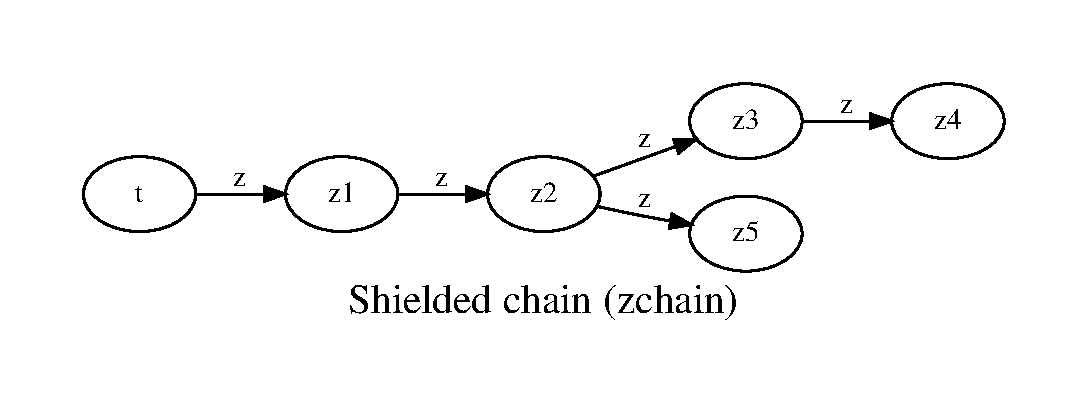
\includegraphics[scale=0.9]{itm-zchain.pdf}

A simpler zchain of only $ t \rightarrow z $ or $ t \rightarrow z \rightarrow z $ does not have enough structure to leak metadata. We need
a structure where we can remove an "inner zutxo" that other things depend on.

The ITM Attack marks $z3$ as invalid via HaveShieldedRequirements() or GetSaplingAnchorAt() returning false when actually the conditions
are valid. When $z4$ transaction is attempted, it will fail since the zk-snark proof will reveal a depedency on $z2$. ITM calls this
a "reverse proof". There is also the possibility of a "forward proof" when z12 allowed the x12 and y12 fails. In that instance, we can
say $ t12 \rightarrow x12 \rightarrow y12 \rightarrow z12 $ with high probability.

These "zchains" are the main objects of attack and study in an \ITM, where it is an iterative process. To summarize, the \ITM requires
a zutxo be spent to attempt to trace it's linkability to other previous ztuxos. An unspent zutxo cannot be analyzed. Additionally, $ t \rightarrow z $ and 
$ z \rightarrow t $ do not currently seem vulnerable. Only $ z \rightarrow z $ transactions can be analyzed, and only the "inside" of the
zchain can leak metadata, the very newest unspent zutxos do not give up metadata.


\nsection{Metaverse Metadata Attacks}

The ITM Attack is a special case of what we name \textbf{Metaverse Metadata Attacks}, applied
to Zcash Protocol shielded transaction graphs.

The term \textbf{Metaverse} is appropriate because alternate possible blockchain histories can be simulated to see what consensus rules would have produced.
By meticulously changing one piece of data at a time, the analyst can use the consensus rules at that moment in blockchain history as an \textbf{oracle}.
In this sense, \textbf{Metaverse} attacks can be classified as \textbf{consensus oracle attacks}, similar to \textbf{compression oracle} attacks and \textbf{padding oracle}
attacks such as \cite{BREACH}, \cite{CRIME} and \cite{HEIST} against SSL/TLS.

While the above attacks are \textbf{side-channel attacks} using the timing response of requests,
Metaverse Metadata Attacks are side-channels that study public chain data and consensus-level
errors in simulations.

As far as the authors know this is a new technique that has not been publicly described.
Blockchain consensus rules can be simulated in a vacuum and the scientific method of changing one variable at a time can be used to extract metadata from privacy coin public data.
There is untold amounts of metadata which can be "mined" from public blockchain data married to OSINT datasources.

\nsection{Sietch: Theory}

\nsubsection{Sietch: Basics}

The ITM Attack relies on the fact that the most common shielded transaction on most currently existing Zcash Protocol blockchains have only 2 outputs $T: z \rightarrow z,z$ and the basic fact that if some metadata can be leaked about one output, if it's \textbf{spent} or \textbf{unspent} or it's range of possible values, it provides a lot of metadata on the other output as well.

If there were 3 outputs, then there would be uncertainty involved, instead of a more direct algebraic relation such as "if one output had amount=5 then the other output had an amount of $total - 5$". When 3 \zaddr outputs are involved, knowing the value of one \zaddr output does not provide as much information on the value of any other particular \zaddr.

This principle obviously increases, as the number of outputs increases, the leakage of
the amount of any one \zaddr input becomes exceedingly less valuable and expensive
metadata to utilize.

By design, Sietch is opt-out and by default all users use it without knowing it, which has worked well.
Sietch makes every individual shielded transaction more complex which creates a harder-to-analyze
transaction graph, helping even users which have custom software that does not use Sietch.

The effect of almost all Hush users using Sietch all the time without knowing it, is a
"herd immunity" against de-anonymization. The price is waiting a few extra seconds
for each transaction and the Hush community feels it is quite well worth it.

Even if some outputs of a transaction are completely de-anonymized, there are so many other
outputs that exact values being transferred cannot be ascertained. This mimics the case
where an infected person cannot easily infect another person with a virus because the people near them
are already in recovery or immune.

\nsubsection{Sietch: Non-Determinism}

In addition to a minimum number of \zaddr outputs, Sietch introduces \textbf{non-determinism}
into Zcash Protocol. Zcash inherited determinism from Bitcoin, where it is a good idea.
In privacy coins, it turns out that determinism can reduce privacy in some situations and it
is not actually a requirement for the cryptocoin to function.

Sietch employs 3 kinds of non-determinism:

\begin{itemize}
\item 1 The order of automatically added \zaddr outputs is random
\item 2 The exact number of automatically added outputs is random
\item 3 The \zaddrs which are sent to are random
\end{itemize}

Hush developers feel that non-determinism is a powerful mitigation against \textbf{Metaverse Attacks}
because when attempting to simulate the blockchain and look for oracles or leak useful bits of metadata,
the outcome of a "test" is no longer deterministic and therefore some attacks will become impractical
or impossible.

\nsection{Sietch: Code In Production}

Sietch uses a default rule of a minimum of 7 \zaddr outputs in a transaction. Because
the average shielded transaction does not spend the input values exactly and there is
a change output, in practice the average Hush transaction has 8 \zaddr outputs.

This is currently not a consensus rule and only enforced at RPC layer. There are
currently various implementations of Sietch in our full node and lite wallets.

Whenever a transaction is made with less than 7 \zaddr outputs, the RPC layer
automatically adds them, which means all software which uses the RPC layer
is protected with absolutely no code changes. Software which uses raw
transactions must take care of this themselves.

This has the practical effect of hiding the number of recipients to the average
transactions on the Hush network. When you see a $ z \rightarrow z,z,z $ transaction
on ZEC mainnet, you can be almost sure it is one \zaddr sending to 2 other \zaddrs and
a change output. It could also be sending to three outputs with no change, with drastically
less probability. This type of transaction is "upgraded" to $ z \rightarrow z_7 $ at a minimum
and so you don't know how many recipients are being sent to, except if it is a large number.
In practice, this obscures most transactions on the network and it is mostly mining pool payouts
which routinely use many \zaddr outputs or other automated software.

Some transactions look like $ t \rightarrow t,t,z,t $ which is a transparent address sending to
two other transparent addresses, one shielded address and a change output. When Sietch is enabled,
this transaction is "upgraded" to $ t \rightarrow t,t,z,t,z_6$ to satisfy the minumum of 7 \zaddr
output rule. Originally the exact amount of value being transferred to the \zaddr would be known,
because all other values in the transaction are transparent and appear on the public blockchain.
But in the "upgraded" transaction we can only ascertain that some amount $A$ was sent and spread
out across 7 outputs, some of which may be of zero value.

In general, Sietch transactions make the job of de-anonymizing a chain much harder at the individual
transaction level, which then builds up into a very strong and complex shielded transaction graph.
The average ZEC mainnet shielded transaction has two outputs and so it's shielded transaction graph
looks like a binary tree, while the Hush blockchain with Sietch looks like a tree that splits into
8 parts at each node. Trying to follow the flow of funds becomes combinatorially impractical and
expensive for even the largest players.

Here we compare what a Zcash (ZEC) mainnet shielded transaction graph looks like, compared to
the shielded transaction graph we would see with \Sietch on the HUSH mainnet. These two graphics
show two \textbf{hops} where we define one hop as $ z \rightarrow z $ and two hops as
$ z \rightarrow z \rightarrow z $ and so on. After a few hops, it's easy to see that the shielded
transaction graph of a \Sietch-enabled blockchain explodes into a "star" of potential avenues for
funds to flow in. A traditional Zcash Protocol chain is a binary tree and that means that if at
any point you can take control of that \zaddr output, you know metadata about a large sub-graph
of the transaction graph, such as seizing an unprotected wallet.dat file from a mobile phone,
laptop or desktop computer. With \Sietch, if one of Alice's friends has their phone seized, there
are still 7 of 8 places where funds could have gone, which may have been 1-7 actual outputs or
some number of outputs automatically added by \Sietch. There is no way to know exactly \textbf{how many}
people received funds except that at most 8 did and we do not know if all funds went to one \zaddr
output and the rest were zero or some combination of funds in multiple \zaddrs .

An attacker is forced to study a much more complex dataset with \Sietch and that is our goal. It
makes each Hush transaction a little fortress in it's own right, and then when we connect many
of these, the entire shielded transaction graph is very resistant to de-anonymization at any given
place. On average, it is strong in every area of this large set of nodes and edges.

After 10 hops Sietch will spread \zaddr funds into potentially $ 8^{10} = 1073741824 $ shielded outputs
on average while the "plain" Zcash Protocol gives a transaction graph of size  $ 2^{10} =  1024  $ on
average.

\begin{center}
\includegraphics[scale=0.420]{zec-graph.pdf}

\includegraphics[scale=0.314]{sietch-graph.pdf}
\end{center}

\nsection{Implementation Details}

We currently have four implementations of Sietch, two running in production, one which was deprecated
and another still in testing. Initial feedback by privacy coin developers pointed out some issues
in our initial implementations, bringing up threat models we did not initially think about.

Originally all Sietch implementations had a fixed list of zaddrs embedded in source code, and these
were randomly added as outputs to \zaddr transactions. This is not ideal, because if the private keys
of those Sietch addresses are compromised, it would be possible to include that data into chain
analysis software and potentially remove the privacy benefits of Sietch. We note that the worst case
is to revert to pre-Sietch privacy.

In repsonse to this, a Hush developer implemented randomized Sietch \zaddrs at run-time, which are
never stored in source code, or on disk. A random seed phrase is generated and then a random \zaddr
is generated from that seedphrase, and then the private key and seed phrase are immediately deleted
from memory. Since every user now generates Sietch \zaddrs in-memory and they are thrown away, it
is essentially impossible to de-anonymize people in bulk. It requires reading memory from individual
nodes to recover those private keys or seedphrases. Currently SilentDragonLite uses this method,
while the \textbf{hushd} full node still uses a fixed set of 200 randomly chosen \zaddrs \cite{SietchRPC}, \cite{SietchHeader}.

We have an implementation that allows \textbf{hushd} to randomly generate Sietch addresses at
run-time which is still in testing, as it makes low-level changes to how \zaddrs are stored in \textbf{wallet.dat} .

We also note that all Sietch outputs are valid and spendable, they are not "fake" and they are not
invalid outputs which are unspendable, because we belive those could be detected and leak metadata.

\nsection{Thoughts On Device Seizure}

Say Alice sent Bob and Charlie funds in a fully shielded transaction with shielded change: $ z \rightarrow z,z,z$ .

Now let us say that Alice and Charlie have their devices seized, wallet.dat's "liberated" and uploaded
into chain analysis software that understands Zcash Protocol and ITM-Style Attacks. Bob is now in a
posistion where his \zaddr is known by the analyst/attacker, the exact amount sent to him in a certain
txid and potentially other metadata in a memo field. All of this data is valuable input which makes
the ITM attack better at it's job, and can often help "complete" partial de-anonymization which was
unable to fully "resolve" the data.

Even without any new attacks, device seizure and uploading wallet.dat contents into blockchain analysis
software poses an enormous threat to privacy coins and so they should design systems that assume this will happen
and to isolate and comparmentalize the damage possible. Sietch provides one such way to provide a safety
and privacy buffer against real-life scenarios.

\nsection{Advice To Zcash Protocol Coins}

Low numbers of \zaddr outputs are bad for privacy, especially 1 or 2. Enforcing at least \textbf{4} likely makes the ITM attack
impractical since there are so many potential ways to swap in and out the remaining inputs. Hush chose \textbf{7} as a security buffer and because the slowdown associated with 7 outputs amounts
to about 5 seconds on modern hardware, when spending a small number of inputs. This seemed like a reasonable amount
of time for users to make a transaction, given that the original Sprout \zaddrs took over a minute to make the simplest
of transactions.

Allowing users to spend huge numbers of inputs at once makes their transactions stand out. GUI wallets and education
need to improve to reduce loss of privacy.

Do not advocate that users post \zaddrs and the txid's and explorer links they are involved in! Educate them to
keep this metadata to private messages, DMs and other non-public places. The fewer people that know your \zaddr,
the better!

\nsubsection{Sapling Consolidation}

Sapling Consolidation is recommended and provides protection against metadata attacks
as well as \textbf{Denial-of-Service} attacks in addition to it's primary function of reducing the size of
wallet.dat files and hence making them much faster to use. \Hush has added \Sietch to our Sapling
Consolidatoin implementation and also made it leak less metadata
by reducing how many inputs it will ever spend at once, which is 8 to match the average number of outputs in \Sietch.
This means that when this feature is turned on, and a node receives a dust attack of many small inputs, the node
will magically clean up after the attack in the background with best practices for every transaction. These transactions
are guaranteed to leave the size of our \textbf{anonymity set} the same or increase it by 1 (if there is no change output).
The original implementation will spend up to 45 inputs at once and always sent to 1 output with fee=0, which trivially
stands out on the network. On the \Hush network, these consolidation transaction look exactly like a very common
$ z \rightarrow z $ with between 1 to 8 inputs and 7 or 8 outputs, blending into a large crowd of transactions which
have the same properties.

\nsection{Future Considerations}

This section considers various new technologies coming down the pipeline and how they interact with existing
and new metadata analysis techniques.

\nsubsection{Shielded Coinbase}

Shielded coinbase seems interesting but leaks a grave amount of metadata tied to the zaddress of the miner, which
can feed into this analysis. We recommend Pirate, Arrow and other coins implementing enforced \zaddr usage
avoid implementing the new \cite{ZIP-213} "Shielded Coinbase". The Hush community does not agree the the final conclusion
of ZIP-213 that it is ok to make the miner \zaddr output public and that only users concerned with "post-quantum"
privacy need to worry about metadata leakage. It gives no recourse to these users, and so in that sense Sietch
can be seen an a valid defense against quantum computers. Further research is required to see what kind of
speed up quantum computers can have on graph theory algorithms that make up the bulk of an \ITM.

Shielded Coinbase will drastiscally reduce privacy of \zaddr miners, because they will re-use the same \zaddr
for every block and it leaks the \zaddr being mined to. The "normal" behavior of mining to a taddr first then
sending to a \zaddr isolates metadata leakage to the taddr. The \zaddr of a miner is never disclosed publicly.
ZIP-213 says miners should make a new address for every block but that simply will not happen because it's optional
and also makes wallet.dat files very large, slower, more annoying to backup, and various other reasons. All privacy
coin research points to the fact that most users only do what is mandatory, they do not go out of there way to do
extra work to get privacy.

By using Timing and Value Analysis with Shielded Coinbase, an analyst can get a much better estimate on the minimum
value a \zaddr likely has and how much funds pass thru it per time interval, as well as txid's to correlate to the
\zaddr. These can all be used as inputs to the ITM Attack, as well.

ZIP-213 is a fascinating academic exercise which could be implemented with better privacy properties but less auditability,
i.e. knowing exactly how much new funds are being mined in each block. Taking into account the ITM Attack in particular
and Metaverse Metadata attacks in general, ZIP-213 will not increase the privacy of a blockchain but potentially decrease
it by infecting the shielded pool with too much metadata leakage.

In summary, Shielded Coinbase was implemented by Electric Coin Company with little practical regard to increasing privacy on their
blockchain, though it is an interesting technical peice of work. Since increased \zaddr usage does not translate into more profits,
it does not seem likely that they will ever have meaningful privacy on Zcash mainnet.
Only Zcash Protocol blockchains which enforce \zaddr usage have a chance at meaningful privacy.

\nsection{Special Thanks}

Special thanks to jl777, zawy, ITM, denioD and Biz for their feedback and all the people in the Hush community
involved in pushing the bleeding edge of privacy tech forward.

\nsection{Acknowledgements}

This is an independently funded work of research with no 3rd party
funding sources. No funding from Electric Coin Company nor Zcash Foundation was received.

\nsection{References}

\begingroup
\hfuzz=2pt
\renewcommand{\section}[2]{}
\renewcommand{\emph}[1]{\textit{#1}}
\printbibliography
\endgroup

\begin{center}
\textbf{Speak And Transact Freely}
\end{center}

\end{document}
